\documentclass[runningheads]{llncs}
\usepackage{graphicx}
\usepackage{lipsum}
\usepackage{amsmath}

\begin{document}

\chapter{[Chapter 4] Evaluation}

\section{TBA}

TBA

\noindent\rule{12cm}{0.4pt}

TODO:


Evaluation of physics engines can be quite challenging, 
especially when quantitative analysis is preferred.
Little work has been done in this area as of now, 
likely due to the complexity, systematic bias, and the lack of needs.

The evaluation of this project is split into three parts: Benchmark selection, Core functionality, and Performance evaluation.

\subsection{Benchmark selection}

Since the functionality evaluations will be largely comparison-based,
I will be choosing at least three open-source physics engines that support similar features to compare against.
The following engines have been found as possible candidates:

\begin{table}[h]
    \centering
    \makebox[\linewidth]{
    \begin{tabular}
    {|c|c|}
    \hline 
    Physics engine                                & Website                                                         \\
    \hline 
    Advanced Simulation Library                   & asl.org.il                                           \\
    Bullet                                        & pybullet.org                                           \\
    Newton Game Dynamics                          & newtondynamics.com/forum/newton.php                      \\
    Open Dynamics Engine                          & www.ode.org                                            \\
    PAL              & www.adrianboeing.com/pal                                \\
    PhysX                                         & www.nvidia.com/en-gb/geforce/technologies/physx        \\
    Project Chrono~                               & projectchrono.org                                      \\
    Siconos                                       & nonsmooth.gricad-pages.univ-grenoble-alpes.fr/siconos  \\
    SOFA & www.sofa-framework.org                                 \\
    Tokamak physics engine                        & github.com/isegal/TokamakPhysics                        \\
    \hline
    \end{tabular}
    }
\end{table}

I plan to further narrow them down by testing if they work in my environment, 
if they have sufficient documentation, 
and if they support the features I am going to compare on.

\subsection{Core functionality}

The functionality will be evaluated through a series of small runtime tests.
The tests are similar to the ones that already existed\cite{seugling2006evaluation}.
Please note that they are preliminary and might be adjusted for clearer visuals.

\subsubsection{Bounce test}

To test whether the engines could handle object collisions, I measure if the momentum and energy are preserved.

Two identical spheres will be placed in a world with no gravity. 
Sphere A, the one on the left, is located at $(0, 0, 0)$, and is moving along the $+$x direction with a velocity of $\SI{1}{\m\per\s}$.
Sphere B, the one on the right, is located at $(\SI{10}{\m}, 0, 0)$, and is moving along the $-$x direction with a velocity of $\SI{1}{\m\per\s}$.
Both spheres have a radius of 1m and a mass of $\SI{1}{\kg}$. The restitution will vary between $0$ and $1$.

\begin{center}
    \makebox[\textwidth]{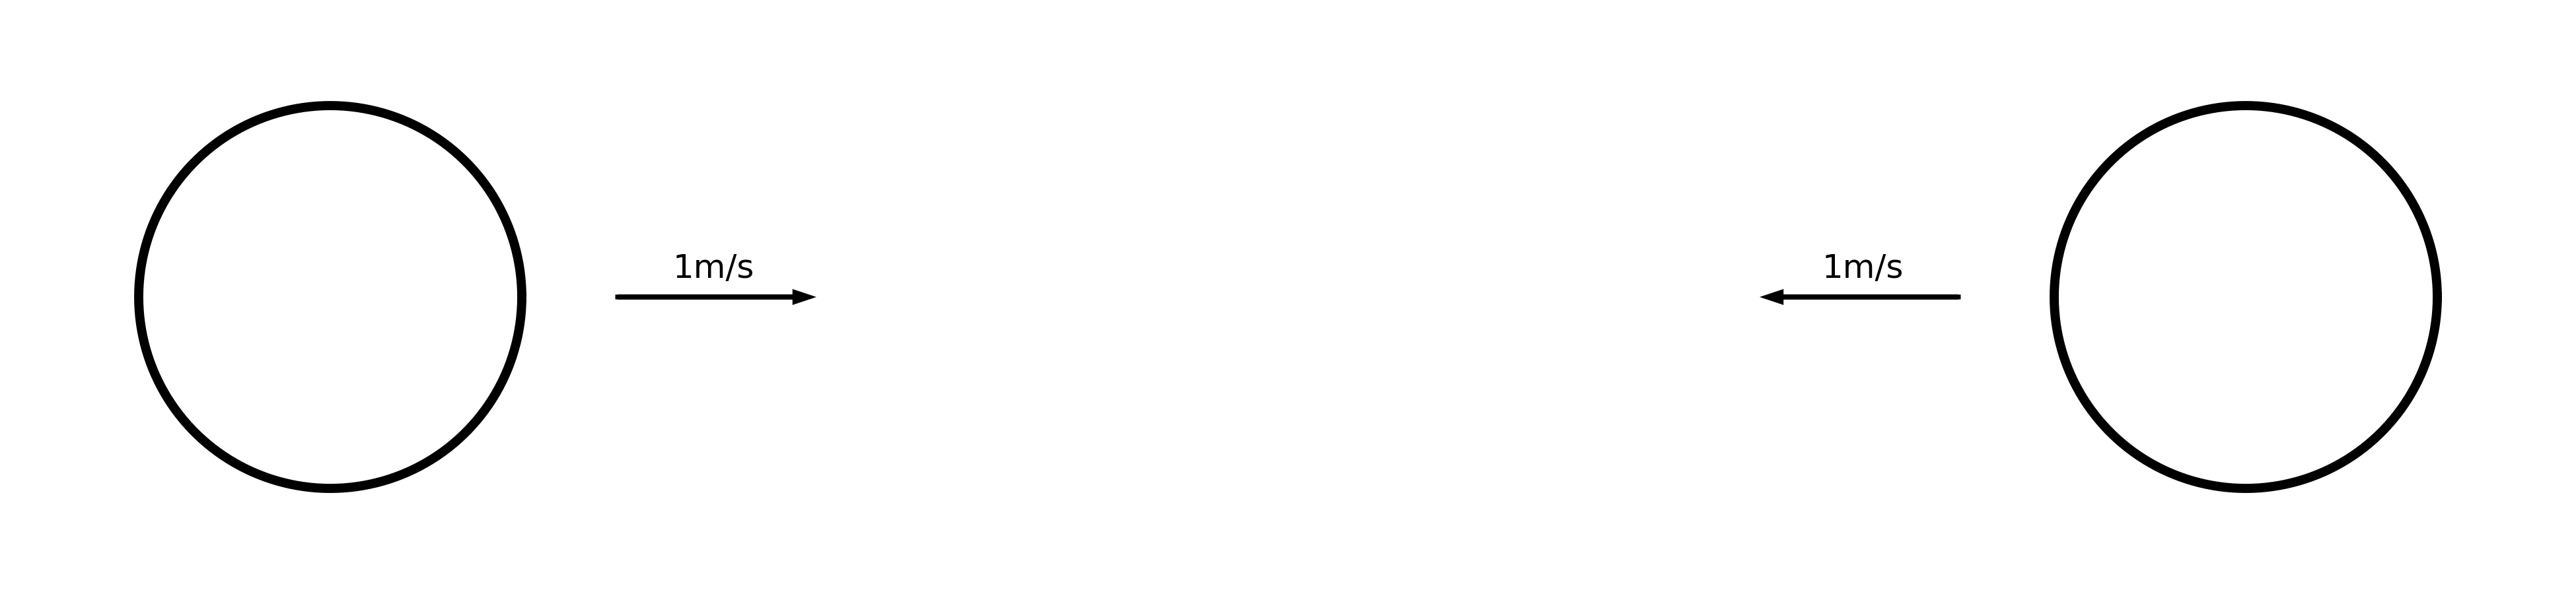
\includegraphics[width=\textwidth]{img1.png}}
  \end{center}

Theoretically, the sum of momentum vectors should stay at $(0, 0, 0)$, and the total energy at $\SI{1}{\J}$.
The actual sum of momentum and total energy, as simulated by the engine, will be plotted against time.
The less these values vary, the more accurate the simulation is.

\subsubsection{Friction test}

Coulomb's Law describes the friction force with the coefficient of friction, $\mu$, which is a constant property of the surface.
If the friction force is $F_f$, the normal force exerted by the surface is $F_n$, then it holds that

\begin{equation}
F_f \leq \mu \times F_n
\end{equation}

Therefore,

\begin{equation}
\frac{F_f}{F_n} \leq \mu
\end{equation}

A box will be placed on a static inclined plane, whose coefficient $\mu = 0.5$.
The angle the surface is tilted by, $\theta$, will gradually increase from 0 to $\frac{\pi}{2}$
A cube of $\SI{1}{\m} \times \SI{1}{\m} \times \SI{1}{\m}$ will be placed on that plane.
A force of gravity $G = \SI{10}{\N}$ will be applied to the cube.

\begin{center}
    \makebox[\textwidth]{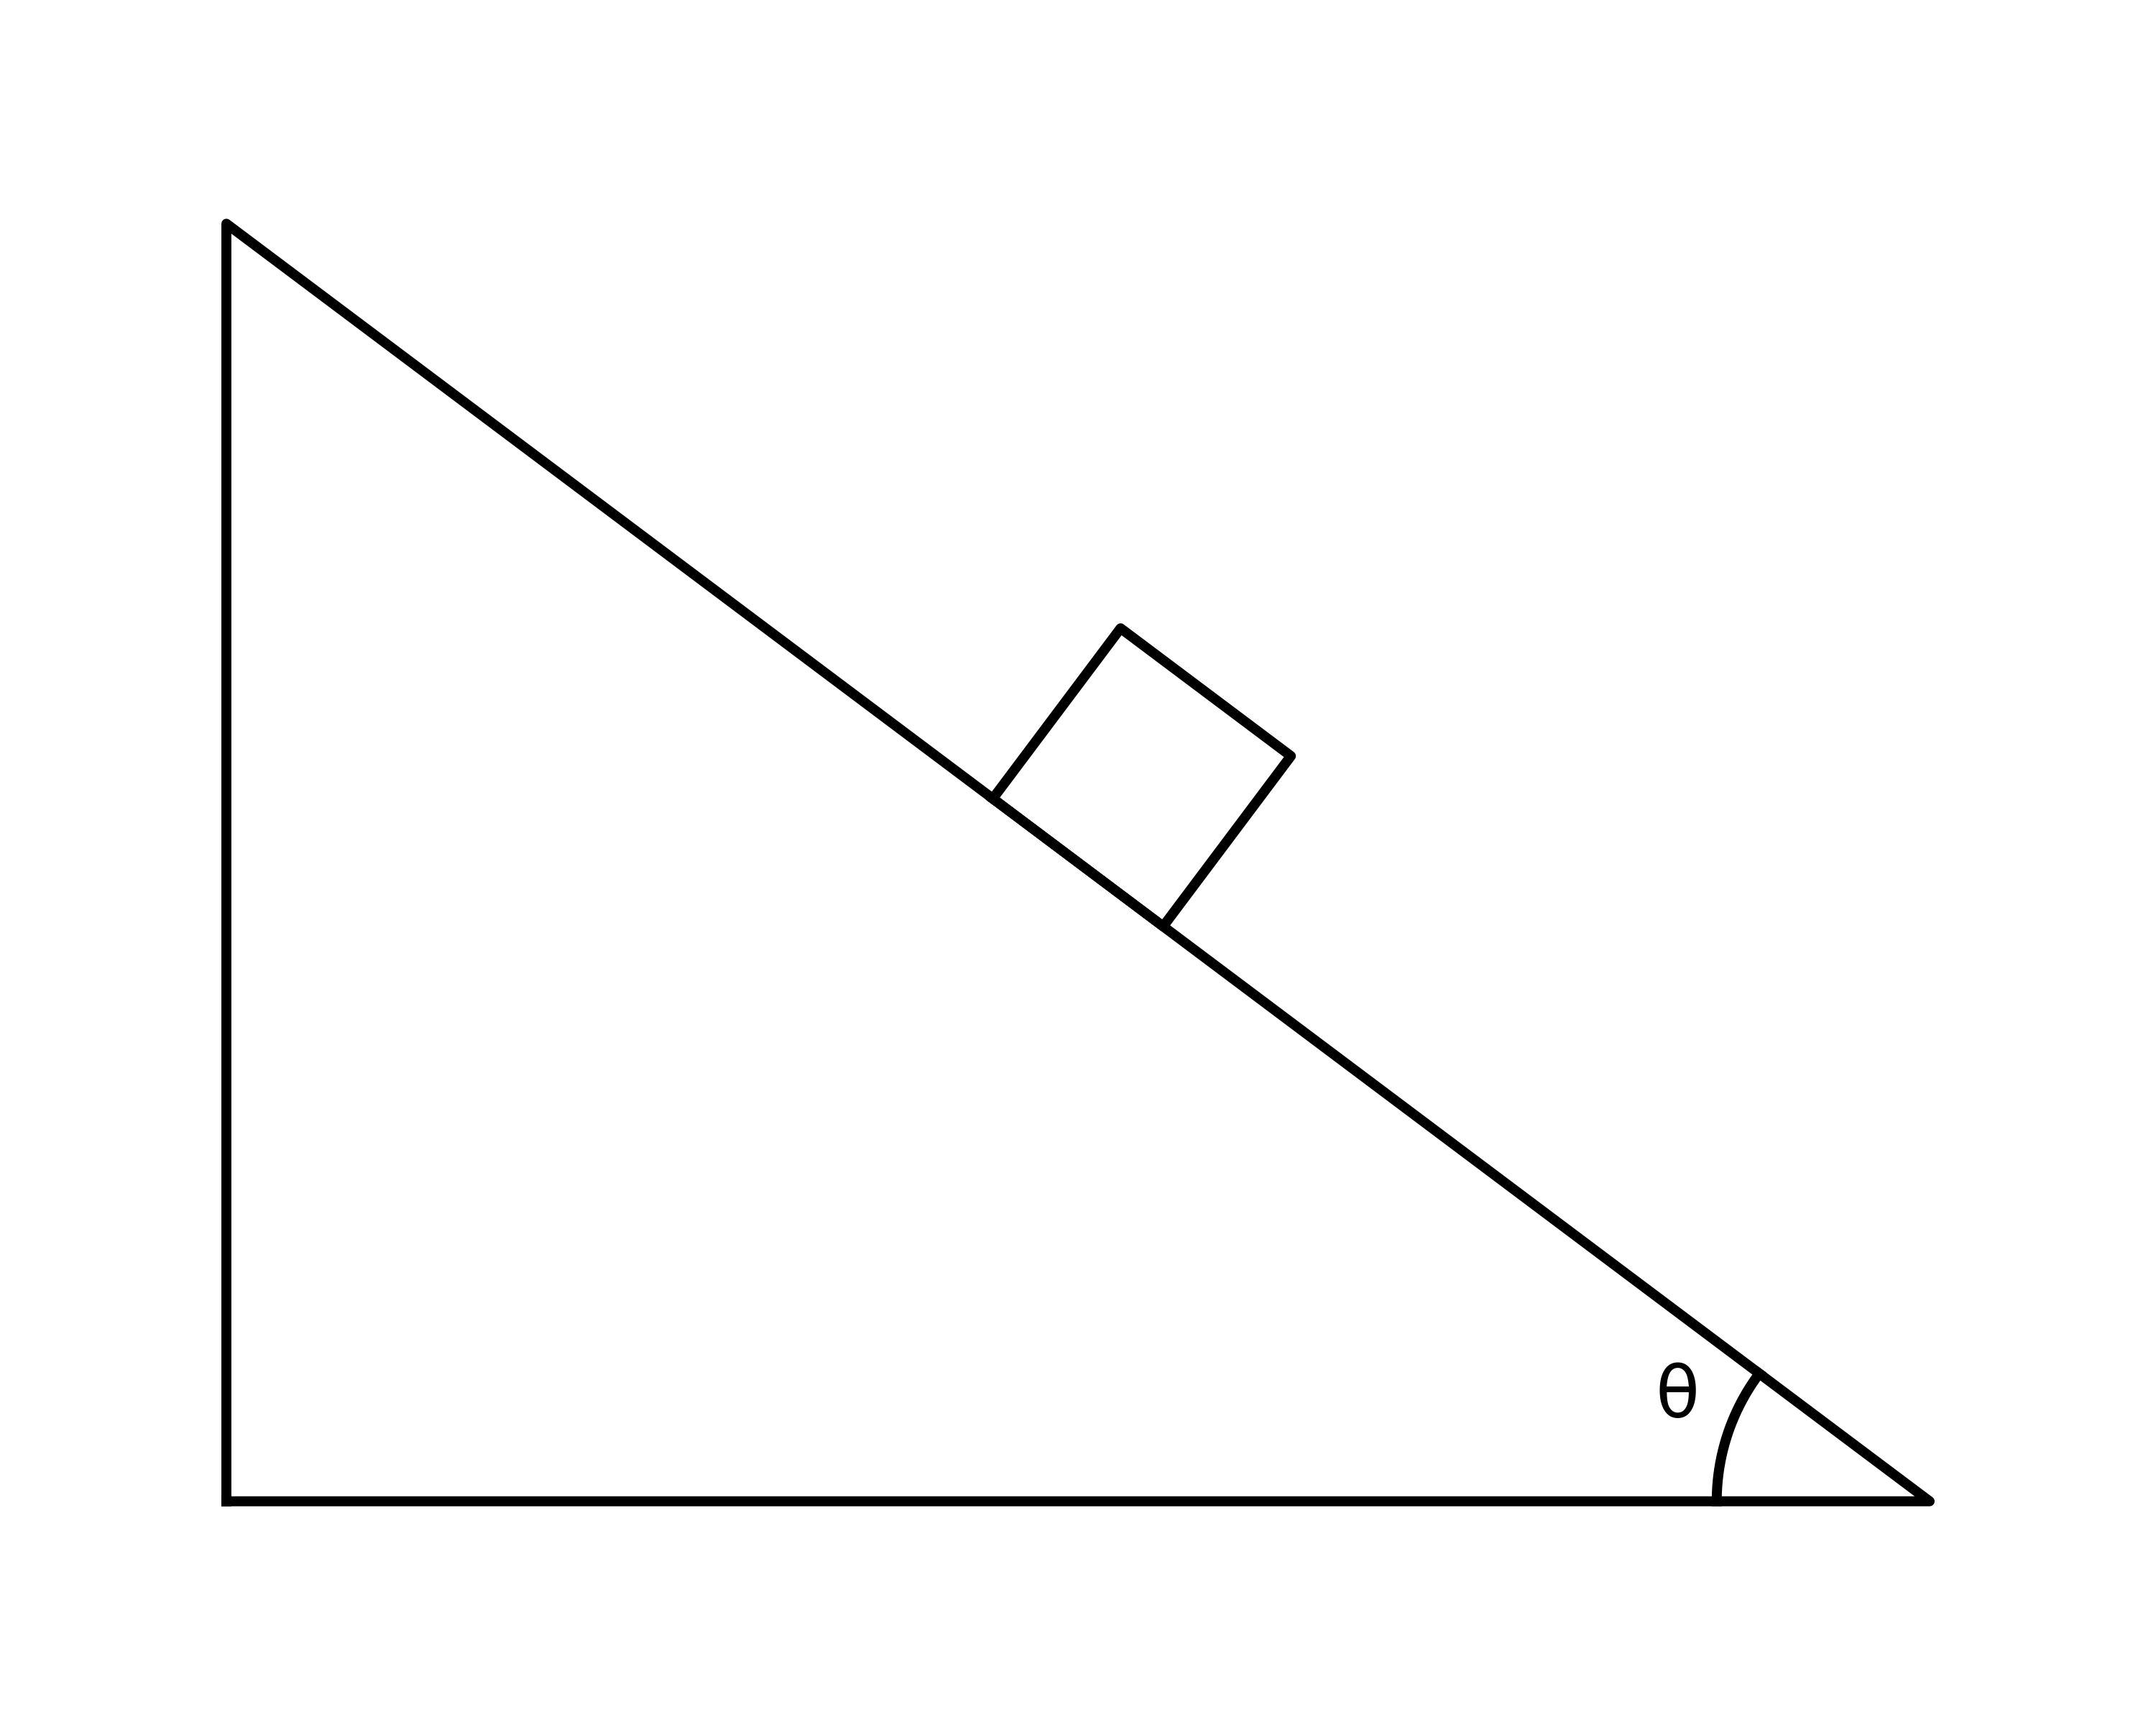
\includegraphics[width=0.5\textwidth]{img2.png}}
  \end{center}

For each angle $\theta$, forces $F_f$ and $F_n$ will be computed as follows.

The normal force is equal to the proportion of gravity perpendicular to the surface:

\begin{equation}
F_n = G \times \cos \theta
\end{equation} 

The friction force is calculated using Newton's First Law:

\begin{equation}
F_f = m \times a - G \times \sin \theta
\end{equation}

Now, $\frac{F_f}{F_n}$ will be plotted against the angle $\theta$. According to Coulomb's Law, it should always stay below $\mu = 0.5$

\subsubsection{Pendulum test}

Have a pendulum setup like in the following figure.
A sphere of radius 1m is attached to a fixed point using a bar of radius $\SI{0.001}{\m}$ and length of $\SI{10}{\m}$.
The initial angle between the bar that connects the sphere and an imaginary vertical line through the fixed point is $\theta$.

\begin{center}
    \makebox[\textwidth]{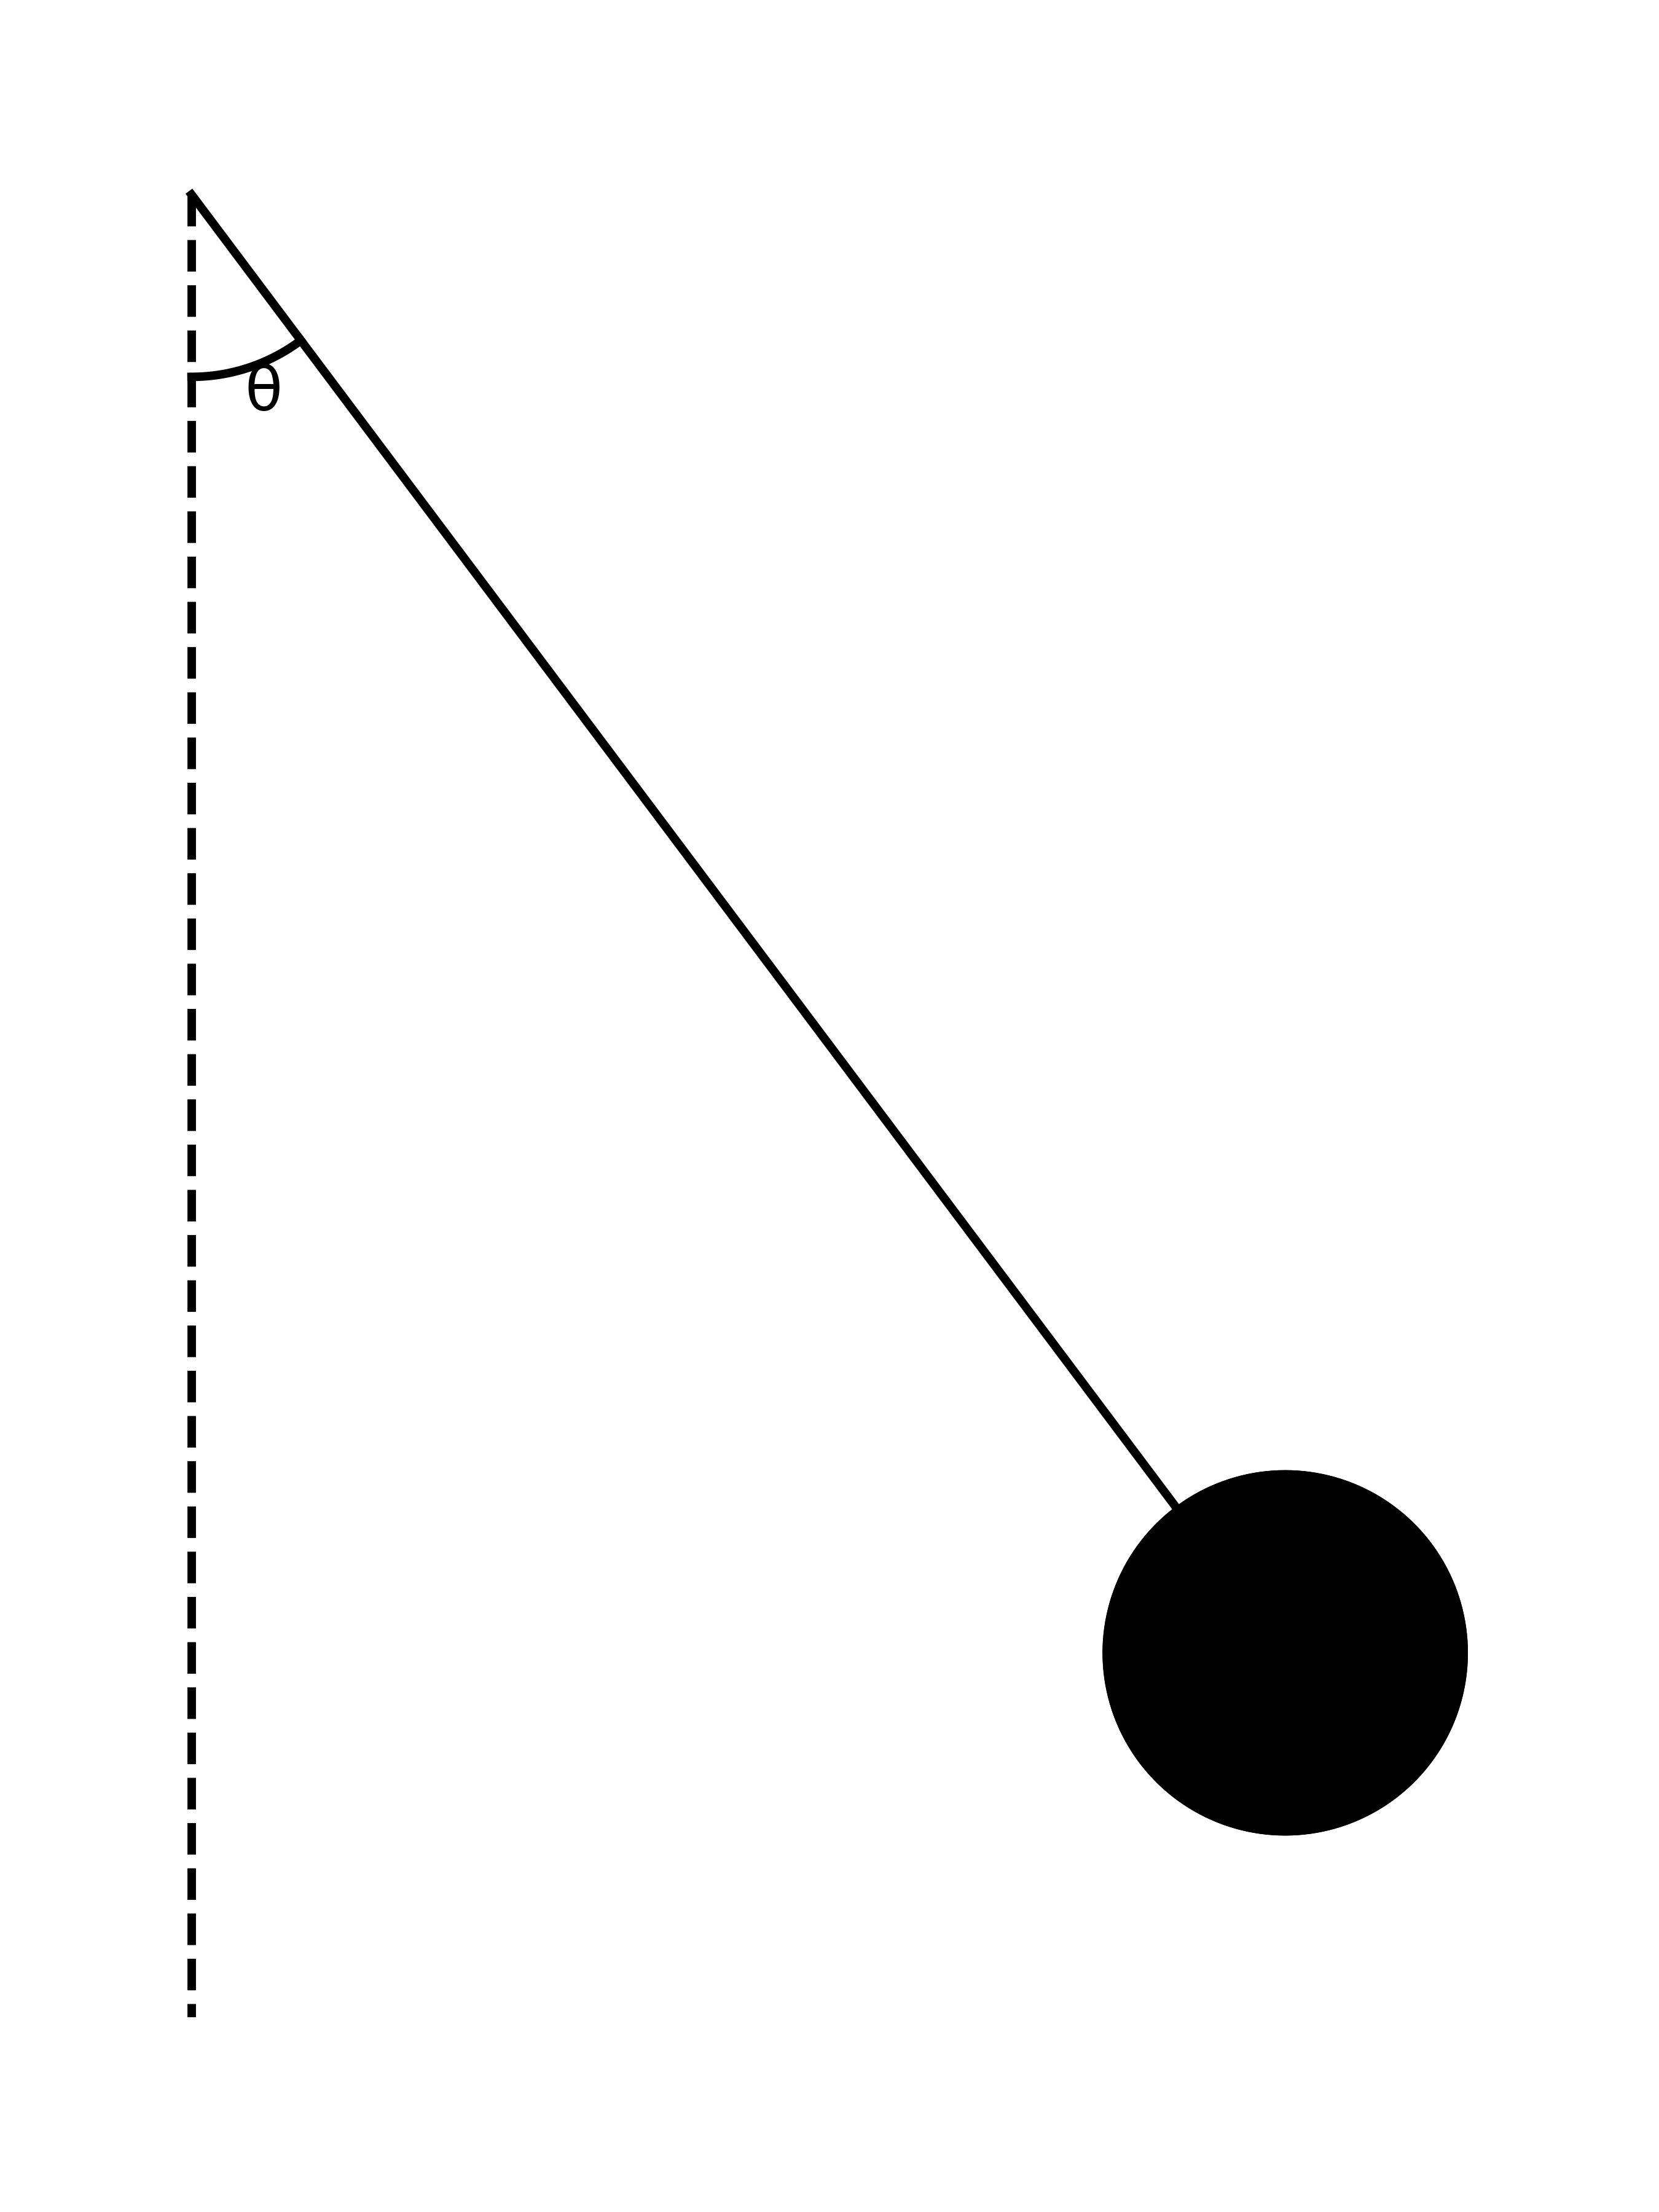
\includegraphics[width=0.3\textwidth]{img3.png}}
  \end{center}

$\theta$ is gradually increased from $5\degree$ to $85\degree$.
For each $\theta$, 
the period of the pendulum is measured by recording the time it takes for the sphere to reach its lowest point $100$ times.

Theoretically, the period of a pendulum is

\begin{equation}
T = 2  \pi \cdot \sqrt{\frac{1}{g}}
\end{equation}

The periods as simulated by the engines will be plotted against the angle $\theta$.

\subsection{Performance evaluation}

This part is considered as an extension. The performance will similarly be measured with a test.

There will be comparisons between my engine and other benchmark engines, as well as between different implementations of my engine.

\subsubsection{Falling test}

a total number of $n$ cubes, all of size $\SI{1}{\m} \times \SI{1}{\m} \times \SI{1}{\m}$, 
are placed at $(0, 0, \SI{2}{\m}), (0, 0, \SI{4}{\m}), \ldots, (0, 0, (n \times 2)\SI{}{\m})$ above a plane of $z = 0$, 
as shown below.
The masses of each cube is chosen uniformly between $\SI{1}{\kg}$ to $\SI{10}{\kg}$, in order to add complexity.

\begin{center}
  \makebox[\textwidth]{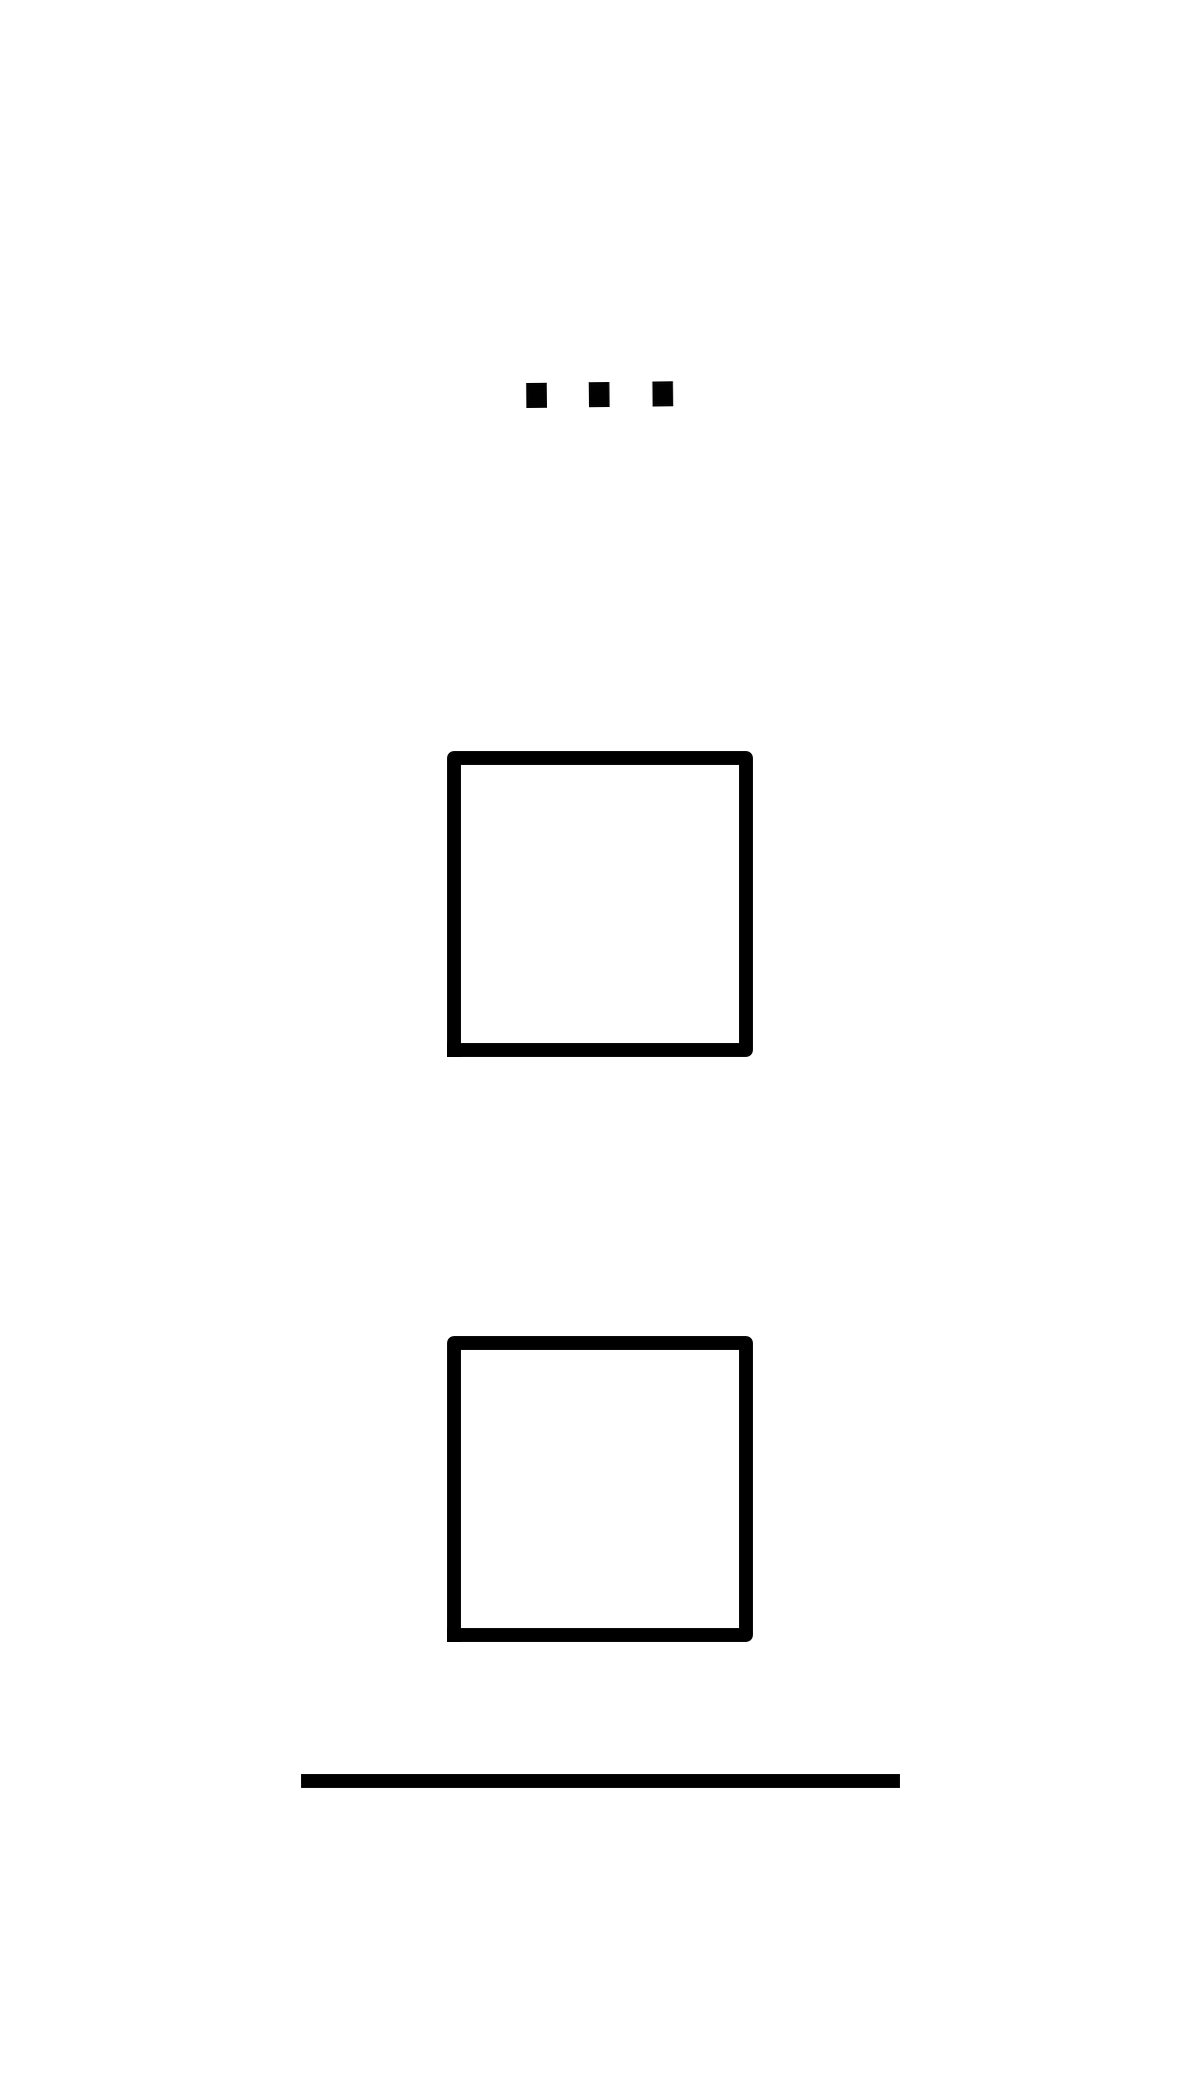
\includegraphics[width=0.3\textwidth]{img4.png}}
\end{center}

The average computational time of a time step is measured and plotted against the number of cubes, $n$.
The average computational time is defined as the average of computational time 
it takes for my machine to simulate the scene in the first $n$ seconds.

\end{document}
